\chapter{Tecnica Ottimizzata}
\label{cap:3}
In questo capitolo viene presentata un'ottimizzazione al problema descritto nel capitolo precedente.
Tale ottimizzazione si basa sul principio delle decomposizioni bilanciate.
Si fa vedere, inoltre, come vengono modificati i precedenti dettagli implementativi ottenendo un miglioramento delle perfomance.

\section{Decomposizioni Bilanciate di un albero}
\label{cap:3 par:1}
Si vuole andare a dimostrare in questa sezione che dato un albero T \`e sempre possibile ricavare una scomposizione bilanciata dell'albero.
\\
Prima di poter enunciare e dimostrare il risultato principale occorre dare delle nozioni preliminari.

\newtheorem{definizione}{Definizione}[section]

\begin{definizione}
	\label{definizioneDeco}
Sia $T_r$ un albero radicato nel nodo r, con k nodi.
Diremo che la coppia (A,B), dove  A e B sono insiemi contenenti i nodi di $T_r$, \`e una decomposizione per l'albero $ T_r $ se:
\begin{itemize}
	\item $| A | + | B | = k$
	\item $A \cap B = \{r\}$.
\end{itemize}
\end{definizione}


\begin{definizione}
\label{lemmaDeco}
Dato un albero $ T $ con $ k $ nodi, diremo che $ (A,B) $ \`e una decomposizione bilanciata se:
\begin{equation*}
	\max{ \{|A| , |B| \} }  \le  f(k)
\end{equation*}
con $ f $ una funzione definita su $ k $.
\end{definizione}





\begin{definizione}
Per ogni nodo $ v $ di un albero $ T $, le diramazioni di $ T $  rispetto a $ v $, sono tutti i sottoalberi massimali di $ T $ non contenenti $ v $. 
Per ogni $ v \in T $, si definisce $\alpha(v)$ come il grado della diramazione di $ v $ con il maggior numero di nodi.\\
Un nodo $ v $ di un albero $ T $ con $ n $ nodi, \`e un nodo centroide se $\alpha(v)\le\frac{n}{2}$.
\end{definizione}\mbox{}

Il centroide di un albero non \`e necessariamente unico, infatti Jordan \cite{jordan1869assemblages}  ha dimostrato che, dato un albero $ T $ con $ n $ nodi:
\begin{enumerate}
	\renewcommand{\labelenumi}{\roman{enumi}}
	\item $ T $ ha un singolo centroide $ v $ e $\alpha(v) < \frac{n}{2}$;
	\item$ T $ ha due nodi centroidi (adiacenti) $v_1$ e $v_2$ tali che $\alpha(v_1) = \alpha(v_2) = \frac{n}{2}$, in questo caso il numero di nodi $ n $ \`e pari.
\end{enumerate}

Esistono diversi algoritmi per la ricerca del centroide, quello utilizzato in questa tesi \`e l'algoritmo di Jordan \cite{jordan1869assemblages} che  ha una complessit\`a temporale lineare nel numero di nodi. \\
Il primo passo da effettuare \`e determinare $\alpha(v)$ per ogni nodo $ v \in T$.\\
Si indica  $\delta(z)$ come il fattore di diramazione di un albero. ossia il numero di nodi incontrati durante una visita DFS (in profondit\`a) effettuata a partire dalla radice $ z $.
Siano $\delta(z_i)$ i fattori di bilanciamento ottenuti da tutte le possibili diramazioni $ i $ di $ T $ unite a $ v $ che non lo contengono, allora, $ \alpha(v) = \max \{\delta(z_i)\} $.

Una volta calcolato il valore di $ \alpha(v) $ $ \forall v \in T $ si verifica per quali valori  risulta $\alpha(v)\le\frac{n}{2}$.\\
Nel caso ci fosse un unico nodo $ v $ che soddisfa la precedente espressione, come in (i),  allora tale nodo rappresenta l'unico  centroide dell'albero $ T $.
Nel caso, invece, ce ne fossero due, come definito in (ii), per esempio $ v_1 $ e $ v_2 $,  l'albero $ T $ conterr\`a due centroidi, rispettivamente $ v_1 $ e $ v_2 $.\\
Nell'esempio \ref{es1} si pu\`o vedere l'applicazione dell'algoritmo per la ricerca del centroide.
	\begin{figure}[htbp]
		\centering
		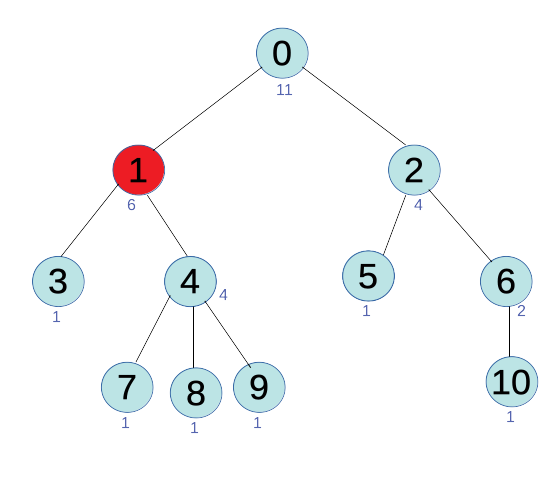
\includegraphics[width=5cm]{capitolo3/grafo2}
		\caption{Albero $ T $  per la ricerca del centroide} 
		\label{fig:2}
\end{figure}
\mbox{}\\

\newtheorem{esempio}[definizione]{Esempio}
\begin{esempio}
	\label{es1}
Si consideri l'albero T in figura \ref{fig:2} per la ricerca del nodo centroide.
Per ogni nodo $ v $ di $ T $ numerato da 0 a 10,  viene calcolato $\alpha(v)$ . \\
Quello che si ottiene \`e :


\begin{center}
	\begin{tabular}{ c c c c c  }
		$\alpha(0) = 6$ & & $\alpha(1) = 7$ & & $\alpha(2) = 5$ \\ 
		$\alpha(3) = 9$ && $\alpha(4) = 10$ &&  $\alpha(5) =  7$ \\  
		$\alpha(6) = 10$ && $\alpha(7) = 10$ && $\alpha(8) = 10$ \\
		$\alpha(9) = 10$ && $\alpha(10) = 10$ &&
	\end{tabular}
\end{center}

Poich\'e $ \left\lfloor\frac{n}{2} \right\rfloor = \left\lfloor \frac{11}{2} \right\rfloor = 5$, l'unico nodo per cui la disuguaglianza risulta vera \`e il nodo 2, infatti $5\le 5$.\\
Poich\`e il numero di nodi \`e dispari certamente questo sar\`a l'unico centroide dell'albero T (figura \ref{fig:2}). 
\demo
\end{esempio}\mbox{}\\

L'ultimo punto da considerare prima di poter enunciare e dimostrare il risultato principale di questa sezione riguarda la definizione di un algoritmo valido per comporre due insiemi di nodi, che chiameremo $ T' $ e $ T'' $, in maniera $ f(k) $-bilanciata.\\
Siano dati in input un albero $ T $, con $ k $ nodi, ed un fattore di bilanciamento definito da una funzione $ f(k) $, poich\'e non considero la radice di $ T $, si avr\'a che $ f(k) = f(k-1) $.
Si suppone inoltre, senza perdita di generalit\`a, che i sottoalberi radicati nei figli della radice $ r $ di $ T $ siano ordinati con ordine non crescente.
Da questo deriva che, supponendo che $ r $ abbia $ n $ figli, vi saranno al pi\`u $  n $ alberi radicati in ciascuno di essi tali che: $ |T_i| \ge |T_{i+1}|$ \ $ \forall i = 1,\dots, n-1 $.\mbox{}\\\\

	\begin{figure}[htbp]
	\centering
	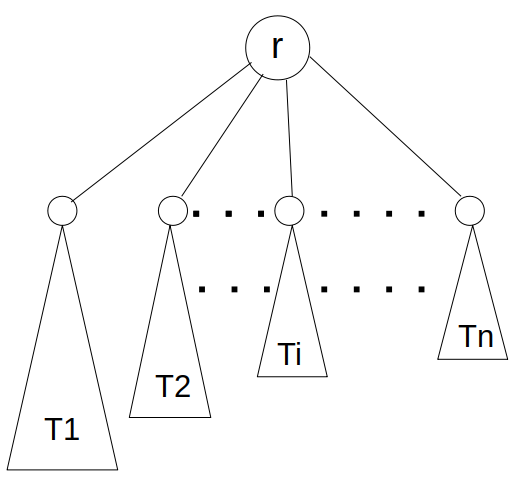
\includegraphics[width=5cm]{capitolo3/grafo3}
	\caption{Esempio di albero $ T $ radicato in $ r $, con $ k $ nodi, valido come input per l'algoritmo \ref{algoritmo1}} 
	\label{fig:3}
\end{figure}
\mbox{}\\

\begin{algorithm}[H]
	\label{algoritmo1}
	\SetAlgoLined
	\caption{Insiemi $ k $-bilanciati}
	\textbf{input} : Albero $ T $ con $ k $ nodi, fattore di bilanciamento $ f(k-1) $;\\
	$ T' , T''\longleftarrow $ due alberi inizialmente senza nodi;\\ 	
	\For{$ i = 1,\dots,n $}
	{
		\If{$ \sum_{j=1}^{i}{|T_j|} > f(k-1) $}
		{
			$ T'\longleftarrow $ sottoalbero di  di $ T $ indotto da $ \{r\} \cup \bigcup_{j=1}^{i-1}V(T_j)$.\\
			$ T''\longleftarrow $ sottoalbero di $ T $ indotto da $ V(T) \diagdown T'$.
		}
		 
}
	\textbf{return} ($ T',T'' $).

\end{algorithm}\mbox{}\\

Una volta concluso l'algoritmo \ref{algoritmo1} si avr\`a una coppia $ (T',T'') $ tale che : $ \max (|T'|,|T''|) \le f(k-1)=f(k) $. 
Viene pertanto rispettata la definizione \ref{lemmaDeco}, perci\`o si ottiene una decomposizione $ f(k) $-bilanciata.

In base a tutte le nozioni fino ad ora discusse si pu\`o dare il seguente risultato\mbox{}\\
.


\newtheorem{teorema1}[definizione]{Teorema}
\begin{teorema1}
	\label{teorema1 cap3 sez1}
Per ogni albero T di k nodi esiste un nodo r di T  tale che l'albero $T_r$, ottenuto radicando T in r, ammette una decomposizione $ (\lfloor \frac{2}{3}(k-1) \rfloor + 1)$-bilanciata ed, inoltre, sia $ (|T'|,|T''|)$ tale decomposizione risulta che il $ \max \{|T'|,|T''|\} \ge 2+ \left\lfloor \frac{(k-1)}{3}\right\rfloor $
\end{teorema1}\mbox{}
\begin{proof}
	
	Sia $ T $ un albero di $ k $ nodi,con $ k>2 $ (per $n\le2$ la propriet\`a \`e banalmente vera) \\
	La prima operazione da compiere \`e individuare il nodo $ r $ di $ T $ su cui si andr\`a poi a radicare il nuovo albero $ T_r $.\\
	Si suppone che tale nodo sia un centroide dell'albero $ T $ quindi si applica l'algoritmo di Jordan per la ricerca del centroide. Senza perdita di generalit\`a si suppone di avere un unico nodo centroide, indicato con $ r $.\\
	Se il centroide $ r $ trovato non corrisponde alla radice dell'albero $ T $, si modifica $ T $ radicandolo in $ r $ e l'albero cos\`i ottenuto verr\`a indicato con $ T_r $. \\ 
	Inoltre, si suppone che i sottoalberi radicati nei figli di r siano ordinati in maniera non crescente rispetto alla loro dimensione.\\
	Si applichi a $ T_r $ l'algoritmo \ref{algoritmo1} precedentemente descritto per definire se \`e possibile ottenere una decomposizione $ f(k) $-bilanciata, con $ f(k) =
	(\lfloor \frac{2}{3}(k-1) \rfloor + 1  $.\\
	Sia $ \{T_i \ | \  i=1,\dots,n\} $ l'insieme dei sottoalberi radicati negli $ n $ figli di $ r $ e si consideri il primo valore di $ i $ tale che l'istruzione $ if $ di riga $ 4 $ nell'algoritmo \ref{algoritmo1} risulti vera (si noti che tale valore di $ i $ esiste sempre dal fatto che per $ i = n $ la condizione \`e verificata).\mbox{}\\\\
	Sia 
	\[ S = \sum_{i=1}^{n}{|T_i|} = (k-1 ) \]\\
	e sia
	\[ x = \sum_{j=1}^{i-1}{|T_j|} \]\\
	Distinguiamo due casi
	\begin{itemize}
	\item $\textbf{ i>2 }$ Si ha che
	\\ 
	\begin{equation}\label{1}
		x+|T_i| > \frac{2}{3}\cdot S
	\end{equation}
\\
	Inoltre sapendo che per costruzione
	\\	
	\begin{equation}\label{2}
	|T_i| \le \frac{S}{i} \le \frac{S}{3}	
	\end{equation}
\\		
	Sottraendo la disequazione \eqref{2} alla \eqref{1} si ottiene che 
	\\
	\begin{equation}\label{3}
	x > \frac{2}{3}\cdot S - \frac{S}{3} = \frac{S}{3}	
	\end{equation}
\\
 	\item $ \textbf{i=2} $ Anche in questo caso come nel precedente vale la disequazione \eqref{1}.\\
 	Inoltre, essendo $ i = 2 $ per costruzione dell'albero $ T $ si pu\`o dire che
 	\\
 	\begin{equation}\label{4}
 	x = |T_1| \ge |T_2| = |T_i|
 	\end{equation}
 	\\
 	Pertanto, sfruttando la disequazione \eqref{4} combinata con la \eqref{1} si ha che
 	\\
 	\begin{equation}\label{5}
 	2x > \frac{2}{3} \cdot S \Rightarrow x > \frac{S}{3}
 	\end{equation}
 \\
	\end{itemize}
Per entrambi i casi otteniamo che 
\\
\[ x > \frac{S}{3} \Rightarrow x \ge \left\lfloor \frac{S}{3}\right\rfloor  + 1 \]
\\
Pertanto si avr\`a che 
\\
\[ \left\lfloor \frac{S}{3}\right\rfloor  + 1 \le x \le \left\lfloor \frac{2}{3}\cdot S \right\rfloor \] 
\\\\
Quindi 
\\
\begin{equation}\label{5}
|T'| = 1+x \le 1 + \left\lfloor \frac{2}{3}\cdot S \right\rfloor = 1 + \left\lfloor \frac{2}{3} \cdot (k-1) \right\rfloor	
\end{equation}
\\
\begin{equation}\label{6}
|T''| = 1 + S - x = 1+S-1 - \left\lfloor \frac{S}{3}\right\rfloor = \left\lceil \frac{2}{3}\cdot S \right\rceil = \left\lceil \frac{2}{3} \cdot (k-1) \right\rceil 	
\end{equation}
\\
Inoltre
\\
\[ |T'| = 1+ x \ge 1+ (1 +  \left\lfloor \frac{S}{3}\right\rfloor ) = 2 +  \left\lfloor \frac{(k-1)}{3}\right\rfloor\]
\\
Poich\`e
\\
 	 \[1 + \left\lfloor \frac{2}{3} \cdot (k-1) \right\rfloor \ge \left\lceil \frac{2}{3} \cdot (k-1) \right\rceil \] 
 	 \\
Possiamo concludere che
\\
\[ 2 +  \left\lfloor \frac{(k-1)}{3}\right\rfloor \le \max\{|T'|,|T''|\} \le 1 + \left\lfloor \frac{2}{3} \cdot (k-1) \right\rfloor \]
 \\
ottenendo perci\'o una decomposizione $ (\lfloor \frac{2}{3}(k-1) \rfloor +1)$-bilanciata, tale che $ \max \{|T'|,|T''|\} \ge 2+ \left\lfloor \frac{(k-1)}{3}\right\rfloor $	 	 
\end{proof}\mbox{}\\\\
 	Nel caso in cui si abbiano due centroidi, la scelta su quale radicare l'albero  \`e deterministica.\\
 	Nel caso in cui gli alberi ottenuti radicando $ T $ in ognuno di essi abbiano strutture differenti, viene scelto quello che tra i due ha una struttura pi\`u piccola.
 	Altrimenti se gli alberi ottenuti sono identici, viene scelto uno dei due in maniera arbitraria.
 	
\section{Algoritmo}
\label{cap:3 par:2}
In questa sezione si vede come \`e stato utilizzato il risultato del paragrafo \ref{cap:3 par:1} per ottimizzare e migliorare l'algoritmo \ref{algoritmo} descritto nel capitolo \ref{cap 2} (paragrafo \ref{section1}).\\
Molto brevemente, quello che si faceva in precedenza era, dato un albero $ T_C $, con $ T $ un albero colorato radicato di $ k $ nodi i cui colori giacciono in $ C $, si procedeva al conteggio delle occorrenze di $ T_C $ nel seguente modo
\[	c(T_c,v)=\frac{1}{\beta_T}\sum_{(u,v)\in E}\sum_{\substack{C' \subset C \\C'' = C \setminus C' \\ |C'|=|T'|, |C''| = |T''|}}c(T'_{C'},v)\cdot c(T''_{C''},u) \]\\
con $ T' $ e $ T'' $ due alberi colorati, radicati rispettivamente in $ v $ ed $ u $ tali che, l'albero $ T' $ avesse un numero di nodi pari ad $ i $, con $ i = 1, \dots , k-1 $, mentre l'albero $ T'' $ avesse un numero di nodi pari a $ k-i $.

In questa nuova versione, invece, $ T_C $ viene suddiviso in due alberi $ T' $ e $ T'' $ tali da  rispettare il principio delle decomposizioni bilanciate e pi\`u nello specifico il teorema \ref{teorema1 cap3 sez1}.\\
Innanzitutto si determina se l'albero $ T_C $ \`e radicato nel proprio centroide, nel caso in cui ci\`o non fosse vero, l'albero $ T_c $ non viene conteggiato.\\
Successivamente vengono individuati due alberi $ T'_{C'} $ e $ T''_{C''} $ radicati entrambi nella radice $ r $ di $ T_C $ e colorati in modo tale che $ C' \cap C'' = c_r $, con $ c_r $ il colore del nodo radice.\\
I due treelet $ T' $ e $ T'' $ saranno tali che $2+ \left\lfloor \frac{(k-1)}{3}  \right\rfloor \le |T'| \le \left\lfloor \frac{2}{3}(k-1) \right\rfloor  +1 $ e $ |T''| = |T| -|T'| $.\\
Come nel caso precedente, l'algoritmo che si utilizza per il conteggio delle occorrenze dei $ k $-treelet colorati in $ G $ \`e dinamico, quindi si procede dai sottoproblemi pi\`u piccoli arrivando a quello pi\`u grande.\\
Anche qui per ogni nodo $ v $ si inizializza $ c(T_{C_0} , v) = 1 $, dove T \`e il treelet di 1 nodo e $ C_0 = \{c_v\} $.
Questa volta, per\`o, per calcolare le occorrenze dei $ k $-treelet radicati in ogni $ v \in V $ di $ G $ non sar\`a necessario aver valutato tutte le occorrenze dei treelet fino a $ k-1 $, ma sar\`a necessario calcolarli fino a $ \left\lfloor \frac{2}{3}(k-1)\right\rfloor +1 $.
Tale conteggio verr\`a eseguito sulla base dell'algoritmo \ref{algoritmo} di sezione \ref{section1}. \\
Per calcolare $ \forall v \in V  $ di $ G $ il numero $ c(T_C,v) $ di occorrenze dei $ k $-treelet (non indotti) radicati in $ v $ isomorfi a $ T $ i cui colori giacciono nell'insieme $ C $, invece, si suddivide $ T $ in $ (T',T'') $ in modo che tale decomposizione risulti bilanciata come descritto in precedenza e si procede al calcolo nel modo seguente\\
\[c(T_C,v) = \frac{1}{\gamma_T}\sum_{\substack{{(T',T'') \ bilanciati}\\{C' \cap C'' = c_r}}} c(T'_{C'},v)\cdot c(T''_{C''},v) \] \\
con $\gamma_T$ la nuova costante di normalizzazione che \`e uguale a $ \binom{p}{q} $, dove $ p  $ \`e il numero di sottoalberi di $ T $ isomorfi al sottoalbero radicato nell'ultimo figlio della radice di $ T' $ e $ q $ il numero di sottoalberi radicati a partire dal primo figlio della radice di $ T'' $ isomorfi al sottoalbero radicato nell'ultimo figlio della radice di $ T' $.
Di seguito l'algoritmo formalmente descritto.\\\\  
\scalebox{0.75}{
\begin{algorithm}[H]
	\label{algoritmo2}
	\SetAlgoLined
	\caption{Fase di costruzione}0
	\textbf{input} : Grafo $ G =(V,E) $, dimensione del treelet $ k $ ,insieme [$ k $] di colori\;		
	\For{$ h = 1$ to $ \left\lfloor \frac{2}{3}(k-1) \right\rfloor +1 $}{
		Si applica l'algoritmo \ref{algoritmo}
	}

	\For{$ v \in V $}{
	\ForEach{$ T : |T| = k $}{
		Si cerca $ c $ il centroide di $ T $;\\
		\If{$ c \ != \ v $} {\textbf{break}; }
		
		\ForEach{$ T' :  2+ \left\lfloor \frac{(k-1)}{3}  \right\rfloor \le |T'| \le \left\lfloor \frac{2}{3}(k-1) \right\rfloor  +1 $}{
			\ForEach{$ T'' : |T''| = |T| - |T'| $}{
		\[c(T_C,v) = \frac{1}{\gamma_T}\sum_{\substack{{(T',T'') \ bilanciati}\\{C' \cap C'' = c_r}}} c(T'_{C'},v)\cdot c(T''_{C''},v)\]	
			}	
		}
	}	
} 	
\end{algorithm}
}\mbox{}\\

Come in algortimo \ref{algoritmo} le occorrenze di $ T $ sono calcolate con un approccio top-down,  per\`o, anche in questo caso nella tesi l'algoritmo \ref{algoritmo2} \'e stato sviluppato bottom-up.
Perci\`o per calcolare le occorrenze dei $ k $-treelet in $ G $, $ \forall v \in V $ di $ G $ si prendono tutte le possibili coppie di alberi colorati $ |T'_{C'}| $ e $ |T''_{C''}| $ radicate in $ v $ tali che: $ 2+ \left\lfloor \frac{(k-1)}{3}  \right\rfloor \le |T'| \le \left\lfloor \frac{2}{3}(k-1) \right\rfloor  +1 $ e $ |T''| = k-|T'| $.
Prima di poterle unire a creare l'albero $ T_C $ bisogna fare le opportune verifiche, ossia:
\begin{itemize}
	\item bisogna verificare che la coppia $ (T',T'') $ sia una decomposizione bilanciata per $ T $.
	Pertanto dovr\`a risultare che $ |T'|-1 $, si va a guardare solo i sottoalberi radicati nei figli della radice, sia  
	$ |T'| - 1 \le \left\lfloor\frac{2}{3}(k-1)\right\rfloor $ e che aggiungendo a tale quantit\`a la cardinalit\`a del sottoalbero radicato nel primo figlio di $ T'' $, chiamata $ t'' $, si abbia che $ |T'| + t'' - 1 \ge \left\lfloor\frac{2}{3}(k-1)\right\rfloor $.
	\item Anche in questo caso bisogner\`a garantire l'ordinamento sulla struttura dell'albero.
	Pertanto non sar\`a possibile unire $ T' $ e $ T'' $ se la dimensione del sottoalbero radicato nell'ultimo figlio della radice di $ T' $ \`e minore del sottoalbero radicato nel primo figlio della radice di $ T'' $.
	\item Bisogna garantire che sia rispettato il vincolo sui colori $ C' \cap C'' = c_v$, ossia i due insiemi condividono esclusivamente in colore della radice $ v $, che \`e la stessa per entrambi. 
	\item bisogna verificare che il nodo $ v $ sia il centroide dell'albero $ T $ risultante dall'unione di $ T' $ e $ T'' $.
\end{itemize}
Queste condizioni sono necessarie affinch\`e l'unione tra gli alberi $ T'_{C'} $ e $ T''_{C''} $ produca un albero valido $ T_C $.

Come si nota, anche in questo caso, i conteggi inizialmente vengono fatti su ogni $ v\in V $, ma poich\`e in questa tesi interessano le occorrenze dei diversi $ k $-treelet su tutto $ G $  sar\'a necessario aggregare gli alberi radicati su ogni $ v $ di $ G $, unendoli a seconda della propria struttura e sommando le rispettive occorrenze.

\section{Dettagli implementativi. Modifica e aggiunte alle rappresentazioni}
\label{cap 3:3}
Anche in questa nuova versione gli oggetti principali manipolati restano i treelet colorati e le occorrenze associate.

Ogni treelet colorato $ T_C = (T,C)$ continua ad avere una rappresentazione unica, memorizzata usando interi da 64 bit.
I bit hanno lo stesso ordinamento della precedente versione.
Quello che cambia, per\`o, \`e la suddivisione dei bit:
\begin{itemize}
	\item i bit da 0-3 contengono un fattore di ``uguaglianza'' nominato $ \textit{equal\_rooted\_tree} $.
	Tale numero \`e pari ad 1 se l'albero ha un solo centroide o due centroidi tali che, gli alberi ottenuti radicando $ T $ in ognuno di essi risultino diversi.
	Mentre \`e pari a  2 se l'albero ha due centroidi tali che, gli alberi ottenuti radicando $ T $ in ognuno di essi risultino uguali.
	\item  i bit da 4-7 contengono il numero di sottoalberi in $ T'' $ radicati a partire dal primo figlio della radice isomorfi al sottoalbero radicato nell'ultimo figlio della radice di $ T' $.
	\item i bit da 8-11 contengono il numero $ q $ necessario nel calcolo binomiale usato in fase di normalizzazione.
	La somma di questa quantit\`a con il numero contenuto nei bit precedenti restituisce l'altro fattore $ p $.
	\item i bit da 12-63 restano invariati alla versione precedente.	  
\end{itemize} 

La struttura dell'albero \`e codificata esattamente come la versione precedente e resta un ordinamento non crescente sull'ordine dei sottoalberi radicati nei figli della radice dell'albero, garantendo cos\`i anche un ordinamento totale sui treelet.\\\\
Alle precedenti operazioni sugli alberi se ne aggiungono delle nuove che sono:
\begin{itemize}
	\item $ \textbf{balance\_merge}(T',T'') $ : fa l'unione di due alberi $ T' $ e $ T'' $ in maniera bilanciata.
	All'interno del metodo viene garantito che tutte le condizioni necessarie affinch\`e l'unione avvenga, descritte nel paragrafo \ref{cap 3:3}, siano verificate.
	\item $ \textbf{normalization\_factor\_balanced}(T) $ : restituisce il fattore di normalizzazione $ \gamma_T $ dell'unione bilanciata.
\end{itemize}\mbox{}\\
Un'altra differenza rispetto la versione precedente riguarda la costruzione della tabelle.
Infatti, seguendo quanto descritto in algoritmo \ref{algoritmo2}, verranno costruite tutte le entrate da 1 a  $ \left\lfloor \frac{2}{3}(k-1) \right\rfloor +1 $ come veniva fatto nella versione precedente.
Mentre non verranno costruite le $ h $ tabelle tali che: $ \left\lfloor \frac{2}{3}(k-1) \right\rfloor +1 < h < k $, ma si proceder\`a direttamente alla costruzione della tabella contenente i $ k $-treelet applicando il metodo $ \textbf{do\_build\_balanced}() $ salvando $ \forall v \in V $ di $ G $ i $ k $-treelet bilanciati raggiungibili con le rispettive occorrenze.
Anche in questa versione i treelet colorati raggiunti $ \forall v \in V $ verranno aggregati e i loro conteggi sommati ed anche in questa versione vengono sfruttati i $ thread $ per permettere dei calcoli pi\`u veloci.